\documentclass{article}
\usepackage{graphicx}
\usepackage{pdflscape}

\title{QRS Detection Algorithm}
\author{Daniel Rodas Bautista\\
115121569}

\begin{document}

\maketitle

\section{Introduction}
%\subsection{The two chosen algorithms}
The aim for this project is to analyse and implement a heart rate monitor on an FPGA board. The most important part for monitoring a heart rate is to correctly detect the QRS complex in the ECG heart signal \cite{principles}. This first report focuses on the software implementation of an algorithm for the detection of the QRS complex. 

Two algorithms were analysed and implemented for reasons that will be explained throughout this report. Initially I worked with the famous Pan Tompkins algorithm since it is the foundation for many other algorithms. Implementing it on software is quite straightforward but since the final goal of this project is to implement it on hardware I ended deciding that it was not fit for this. 

\section{Pan Tompkins Algorithm}

\subsection{Description of the algorithm}

The algorithm is divided into two main parts \cite{pan}. First there is a preprocessing stage followed by the decision stage. The preprocessing stage is made up of several linear filters and one non-linear filter. In principle the final signal of this stage corresponds to the energy of the initial signal. First there is a band-path filter to get rid of the noise. This is followed by a differentiator which accentuates the characteristic  slope of the QRS complex. This signal is then squared (this is the non-linear filter) after which a moving window average, i.e. an integrator, is applied. 

The actual detection stage uses a double threshold technique which is applied both to the output of the integrator as well as the output of the differentiator. A QRS complex is said to be detected only when it has been detected in both signals. Moreover the algorithm keeps track of the last eight RR intervals, i.e. the interval between two QRS peaks. Actually two different RR intervals are memorized but for simplicity in this report I will only mention one. There is a main threshold and if the signal is higher than it and it lays in a valid RR interval then this peak is detected as a valid QRS peak. In the other hand if no valid peak is found in a valid interval then a search-back method is performed by using the second threshold (which is obviously lower than the first one). 

\subsection{Implementation}

The implementation found in \cite{hooman} was the starting basis for the implementation I developed. I decided to simplify the implementation and use only one type of band-path IIR filter for filtering the noise. The detection stage was completely re-done with a more simple approach.

\begin{figure}%[p]
        \centering
        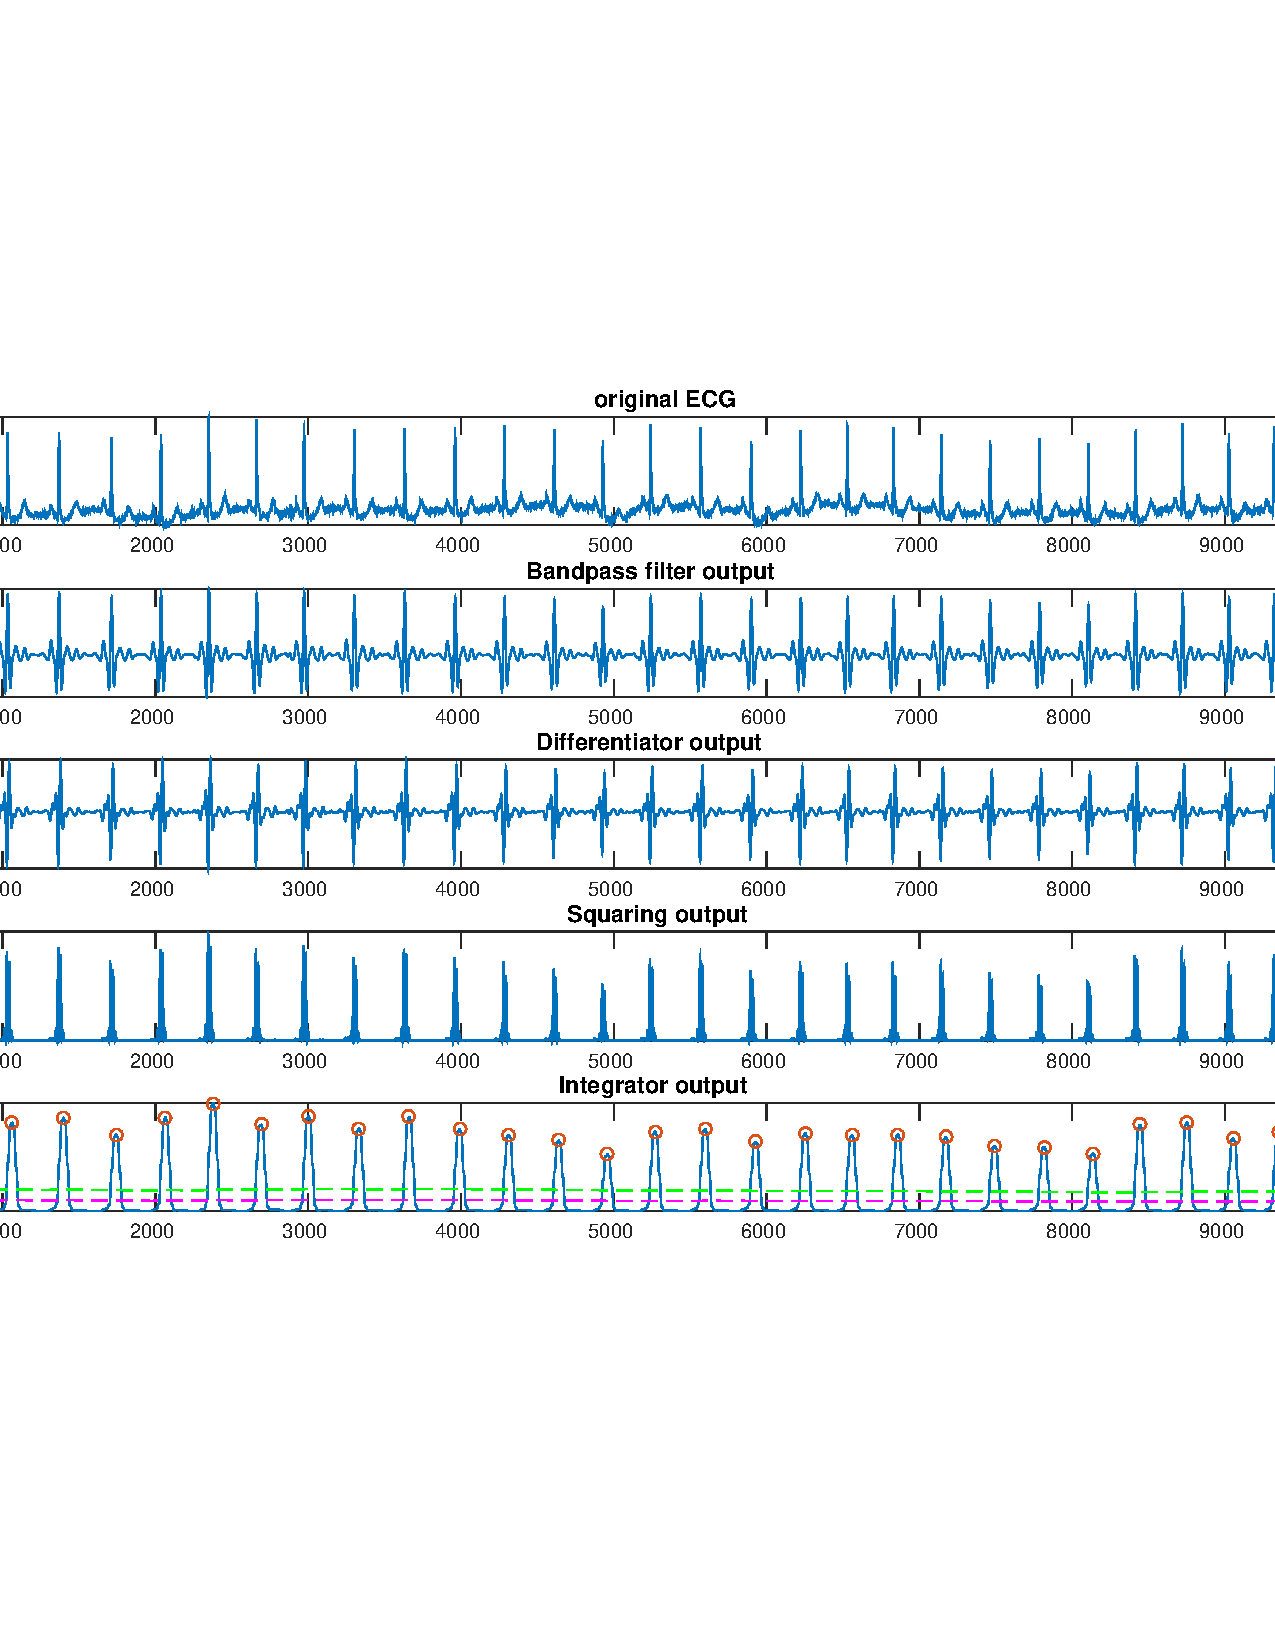
\includegraphics[scale=0.4]{./figs/pan_tompkins30s.pdf}
        \caption{Signal at the various steps of the Pan Tompkins Algorithm}
        \label{fig:pan}
\end{figure}

The Pan Tompkins algorithm is quite straightforward to implement in software but it uses IIR filters, a non-trivial detection mechanism and this results in complex hardware. For this reason I decided to go against using this particular algorithm for my project.

\section{Novel Real-Time Low Complexity Algorithm}

\subsection{Description of the algorithm}

The algorithm is proposed in \cite{rivas}. This is a much simpler algorithm in terms of computational power. The preprocessing stage uses less and simpler filter. The processing or detection stage is implemented with a three state finite state machine (FSM).

Preprocessing is made first by a differentiator, followed by an integrator, finishing with a square function. The differentiator is implemented using a simpler difference equation than the one used in the previous algorithm thus making it much easier to implement in hardware. The integrator uses a window equal to eight (with a sampling frequency of 360 Sa/s) which is a power of two and thus the division (in the average equation) can be easily implemented by a shifter in hardware. Not only does this algorithm uses less filters but they are simpler to implement.

Detection is based on adaptive thresholding. There is only one threshold in this case and it is only applied to the final signal from the preprocessing stage but it adapts to the signal. As mentioned before the detector is a FSM with three states. There is a counter running and it's value is the decisive value in two of the states. During the first state the FSM looks for the highest value in the signal which is then saved as a peak, it goes to the next state when the value of the counter is higher than the minimum feasible RR interval (200ms) plus the standard duration of the QRS complex (60ms). Then the counter is set to a value equal to the current signal index minus the index of the previously found peak. The second state simply keeps the counter going  until the value of the counter is higher than the minimum RR interval. This is where the threshold is set to the average value of all the previous peaks. In the final state the FSM looks for a value of the signal higher than the threshold, in the meantime the threshold is decreased exponentially. 

\subsection{Implementation}

The novel algorithm was implemented on matlab keeping true to it's real time nature by analyzing one sample after the other. 

\begin{figure}%[p]
        \centering
        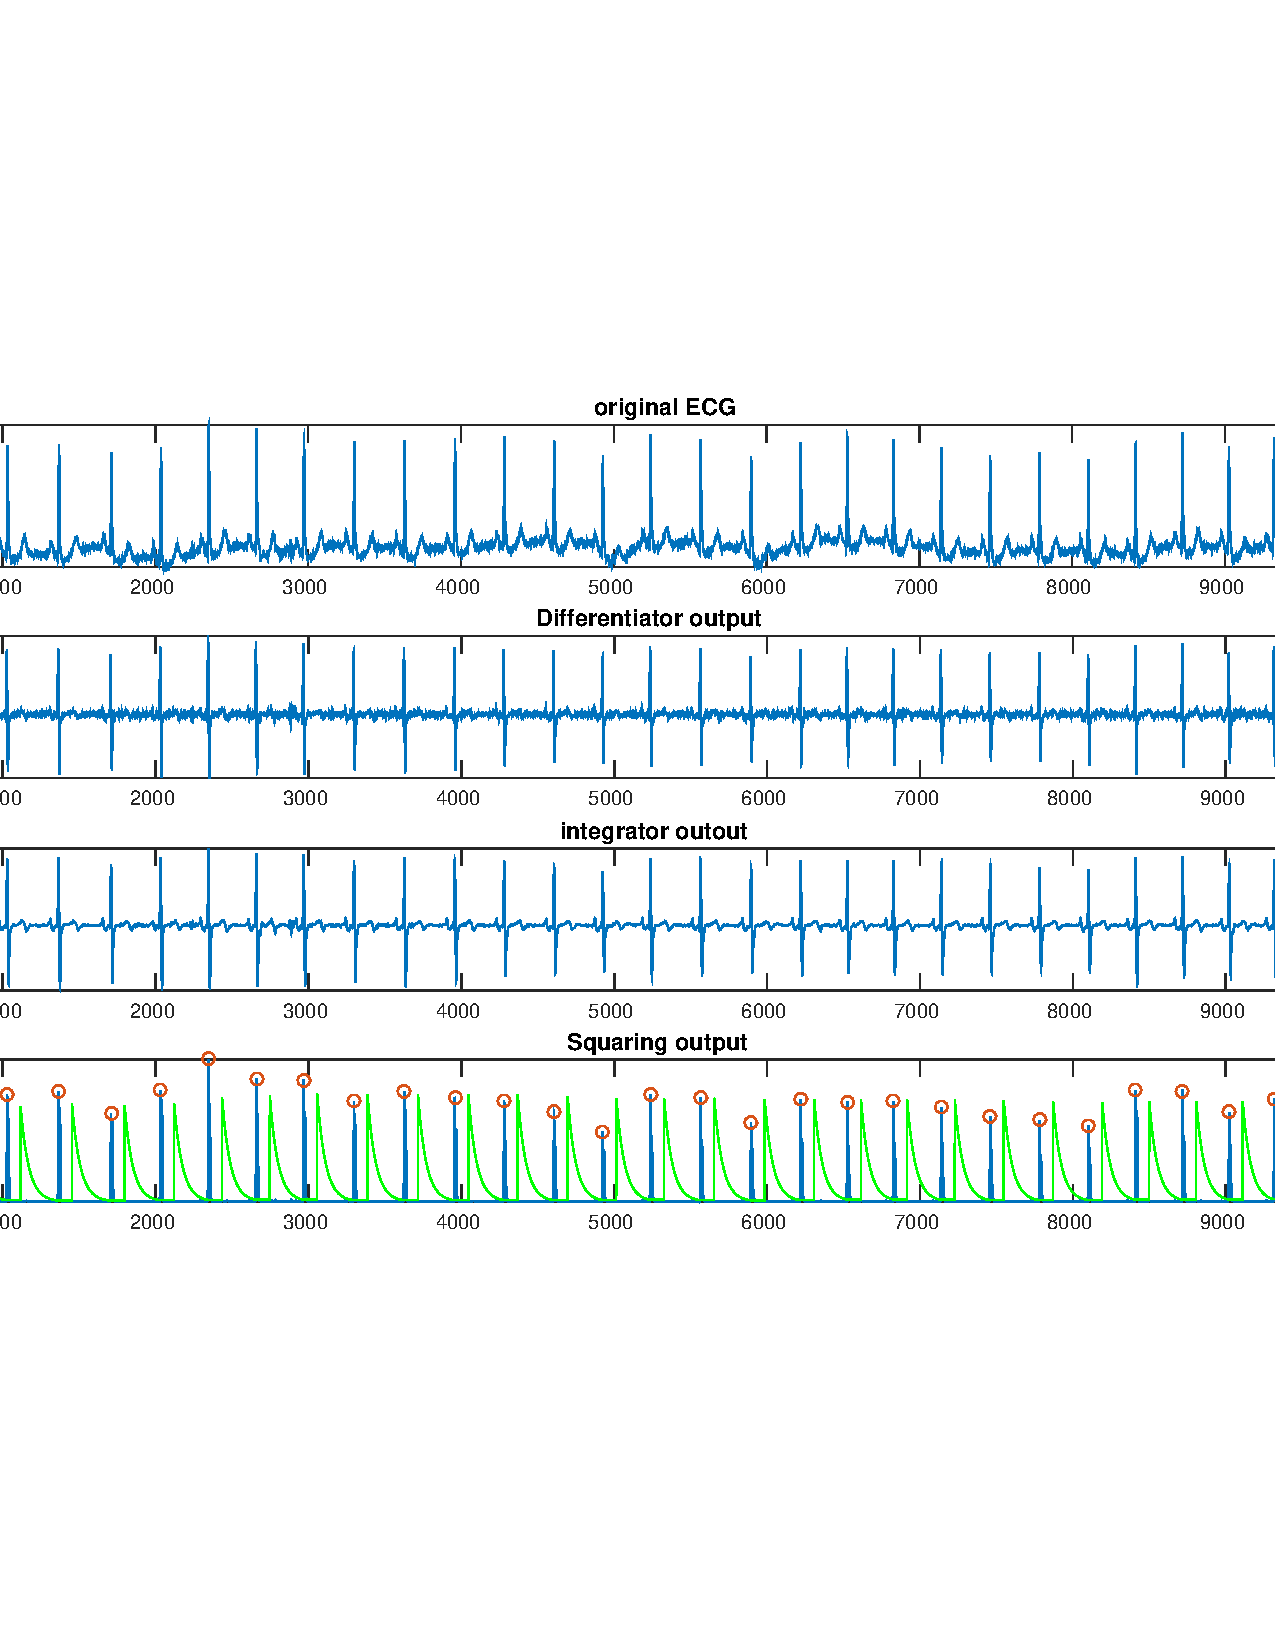
\includegraphics[scale=0.4]{./figs/rivas30.pdf}
        \caption{Signal at the various steps of the Proposed Algorithm}
        \label{fig:rivas}
\end{figure}

\begin{figure}%[p]
        \centering
        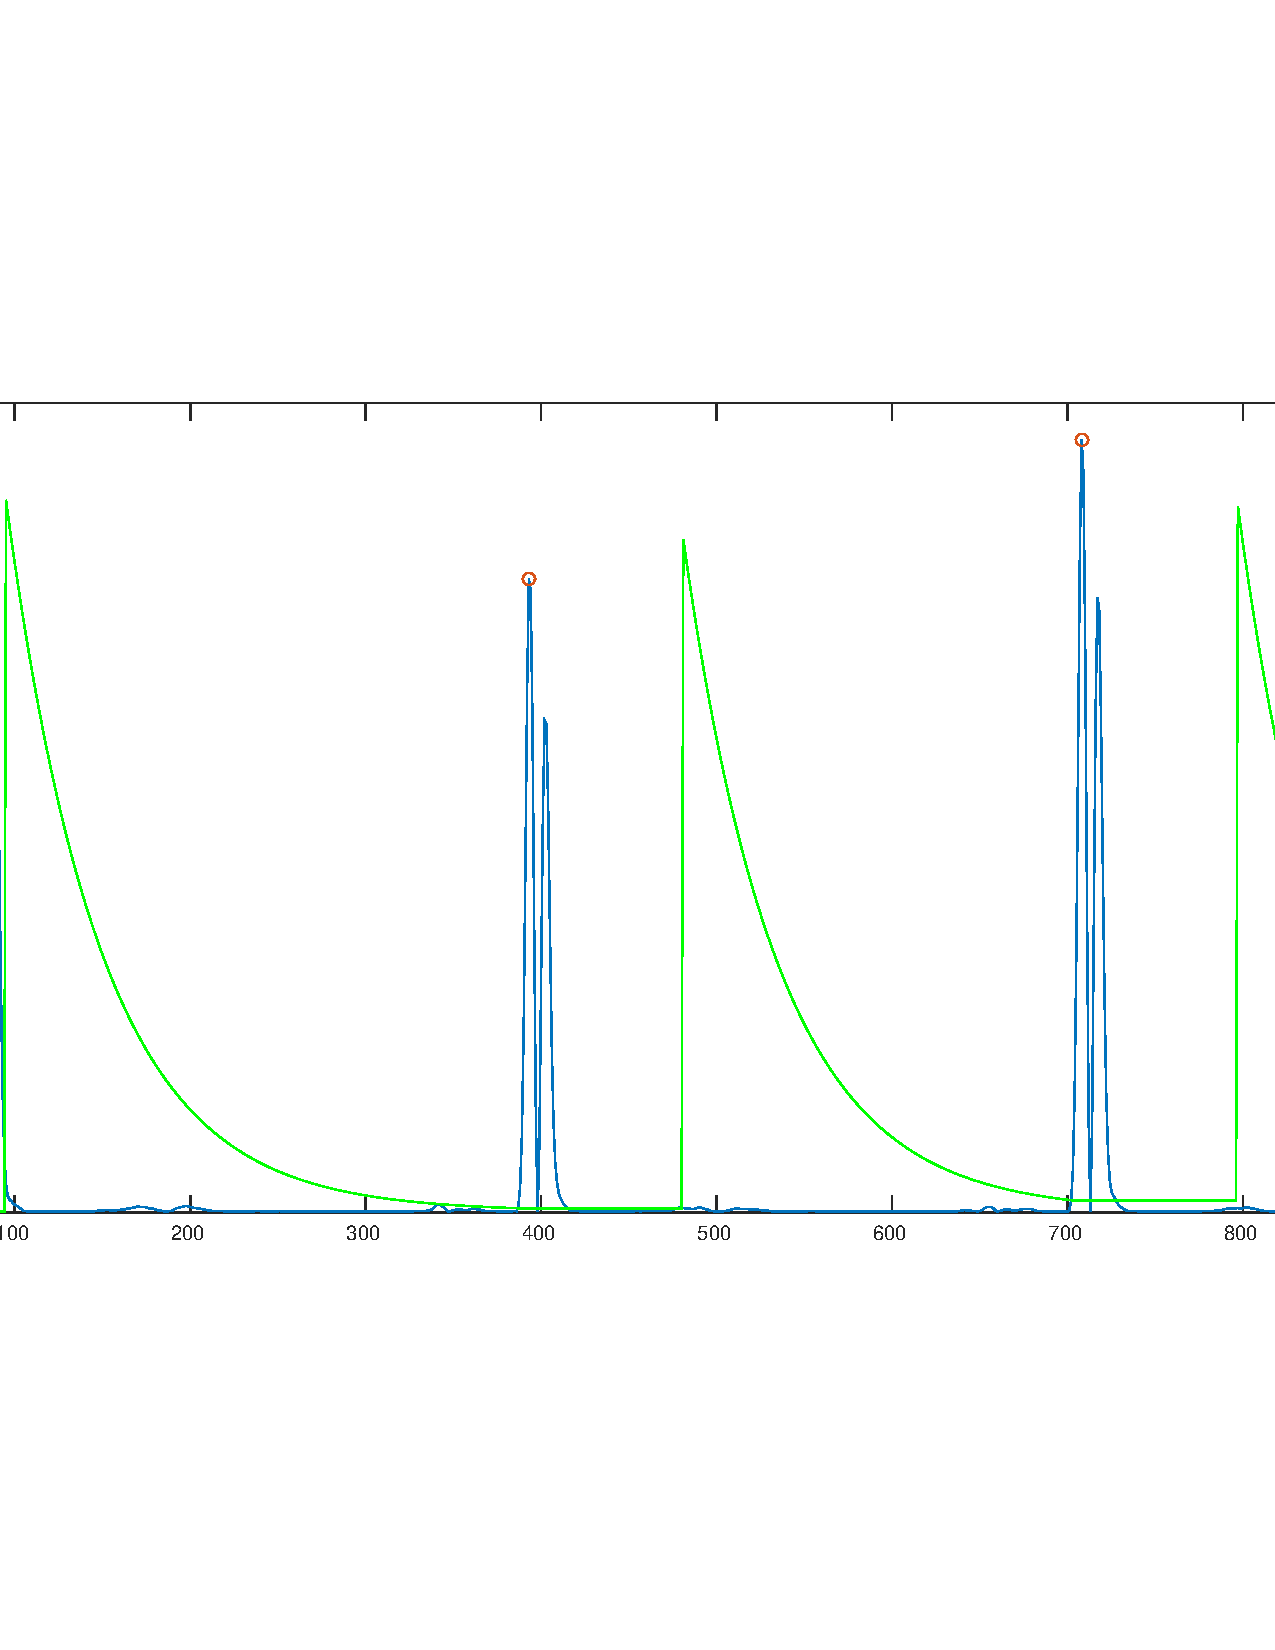
\includegraphics[scale=0.4]{./figs/rivas_closeup.pdf}
        \caption{Close up of the final output signal}
        \label{fig:rivasclose}
\end{figure}

\section{Future Work} %RTL 

\bibliographystyle{plain}
\bibliography{./biblio}

%\section{appendix} %Scripts?

\end{document}
